
\section{Models}
Multiple references are introduced.:\cite{1,2,3}

\begin{figure}[htbp]
	\centering        %居中
	\subfigure[name of the subfigure]{      %第一张子图
		\begin{minipage}{7cm}
			\centering                   %子图居中
			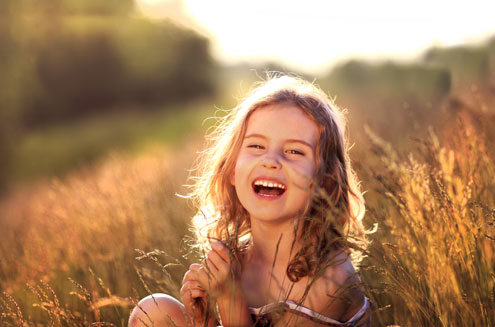
\includegraphics[scale=0.4]{one_3.jpg}          %以pic.jpg的0.5倍大小输出
		\end{minipage}}
	\subfigure[name of the subfigure]{          %第二张子图
		\begin{minipage}{7cm}
			\centering                                                          %子图居中
			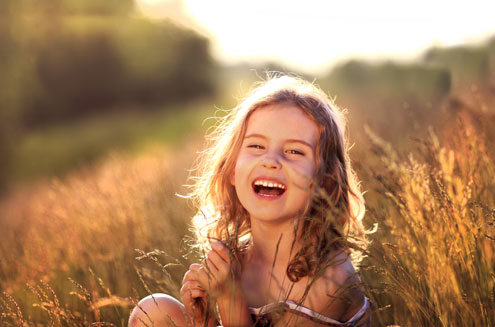
\includegraphics[scale=0.4]{one_3.jpg}         %以pic.jpg的0.5倍大小输出
		\end{minipage}}
	\caption{the figure} %          %大图名称
	\label{fig:123}      %图片引用标记
\end{figure}

Refer to the test for Figure \ref{fig:123}


\begin{figure}[h]
	\small
	\centering
	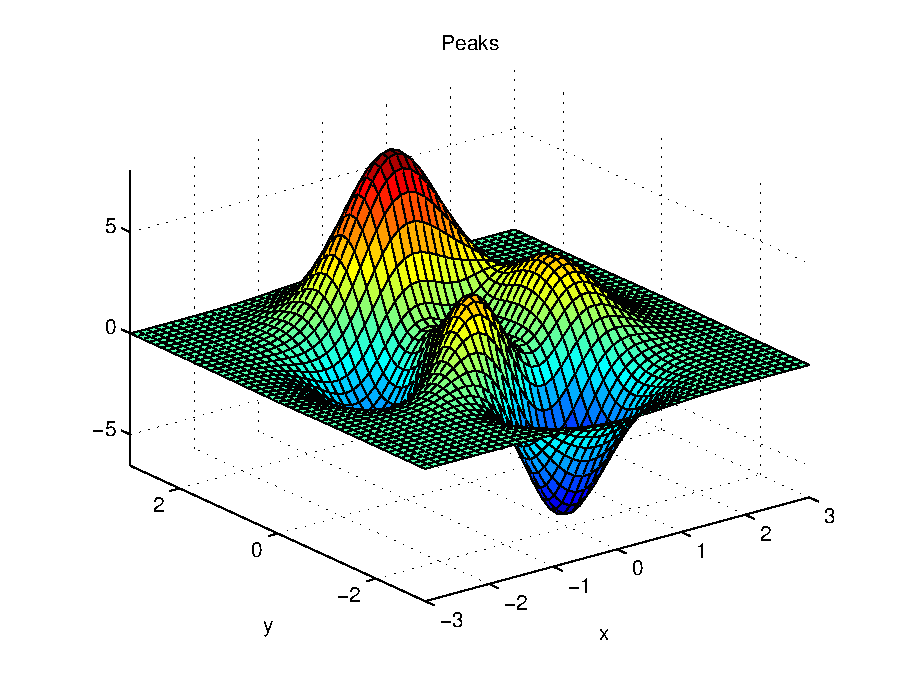
\includegraphics[width=12cm]{mcmthesis-aaa.eps}
	\caption{aa} \label{fig:aa}
\end{figure}





\begin{equation}
a^2 \label{aa1}
\end{equation}
about this eqref \eqref{aa1}

